
\section*{Review}

\frame{
  \frametitle{Review Question \#1}

  If the price of an airplane ticket is $\$300$, then the airline
  sells $2,000$\ tickets.  For {\blue each dollar}\ the airline
  increases the price, it {\blue sells $10$ fewer tickets}.
  \gap

  \begin{itemize}
  \item[\red(1)] 
    If the price is $\$400$, how many tickets does the airline sell?
    \begin{center}
      A$=2000$
      \quad 
      B$= 1000$
      \quad 
      C$= 3000$
      \quad 
      D$= 1990$
      \quad 
      E$= 2400$
      \pause
      \quad
      \fbox{B}
    \end{center}
    \bigskip

    \item[\red(2)]
      If the price is \$$(300+{\blue n})$, how many tickets does
      the airline sell? 
      \begin{center}
        A$=2000-{\blue n}$
        \quad 
        B$= 2000+10{\blue n}$
        \quad 
        C$= 2000-10{\blue n}$
        \quad 
        D$ = 2000/{\blue n}$
        \pause
        \quad
        \fbox{C}
      \end{center}
      \bigskip

    \item[\red(3)]
      If the price is \$${\red x}$, how many tickets does the airline sell?
      \begin{center}
        A$=2000+10{\red x}$
        \quad 
        B$= 2000-10{\red x}$
        \quad 
        C$= 5000-10{\red x}$
        \quad 
        D$= 1000+10{\red x}$
        \pause
        \quad
        \fbox{C}
      \end{center}
      \bigskip
  \end{itemize}

}


\if0
\frame{
  \frametitle{Review Question \#2\ (HW13 \#9)}
  \vspace*{-1em}

  \begin{center}
    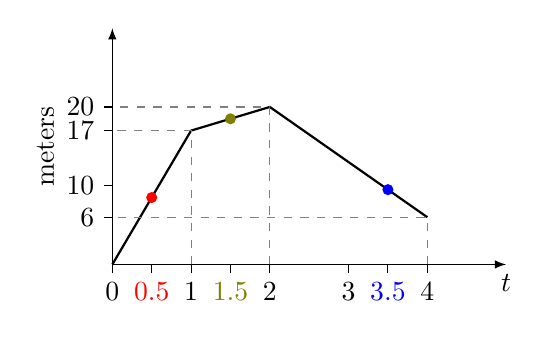
\begin{tikzpicture}[x=10mm,y=1mm,>=latex]
      \draw[thin,black,->] (0,0) -- (5,0) node[below] {$t$};
      \draw[thin,black,->] (0,0) -- (0,30);
      \node[rotate=90] at (-0.85,15) {meters};
      % ticks:
      \foreach \x in {0,1,2,3,4}
      {
        \draw[thin,black] (\x,0) -- (\x,-3pt) node[below] {$\x$};
      }
      \foreach \y in {6,10,17,20}
      {
        \draw[thin,black] (0,\y) -- (-3pt,\y) node[left] {$\y$};
      }
      \draw[thick,black] (0,0) -- (1,17) -- (2,20) -- (4,6);
      \draw[gray,dashed] (1,0) -- (1,17) -- (0,17);
      \draw[gray,dashed] (2,0) -- (2,20) -- (0,20);
      \draw[gray,dashed] (4,0) -- (4,6) -- (0,6);
      %
      \uncover<2->{\fill[red] (0.5,8.5) circle (2pt);}
      \uncover<2->{\draw[thin,black] (0.5,0) -- (0.5,-3pt) node[below,red] {$0.5$};}
      \uncover<4->{\fill[red!50!green] (1.5,18.5) circle (2pt);}
      \uncover<4->{\draw[thin,black] (1.5,0) -- (1.5,-3pt) node[below,red!50!green] {$1.5$};}
      \uncover<6->{\fill[blue] (3.5,9.5) circle (2pt);}
      \uncover<6->{\draw[thin,black] (3.5,0) -- (3.5,-3pt) node[below,blue] {$3.5$};}
    \end{tikzpicture}
  \end{center}
  \vspace*{-2em}

  \begin{align*}
    \uncover<2->{
    \text{speed at {\red$0.5$}} 
    }
    \uncover<3->{
    & = \frac{\text{dist.\ gone betw.\ $t=0$ and $t=1$}}{1\
      \text{sec}}
      = \frac{17-0\ \text{meters}}{1\ \text{sec}}
      = 17\ \text{m}/\text{s}
      }\\
    \uncover<4->{
    \text{speed at {\redgreen$1.5$}} 
    }
    \uncover<5->{
    & = \frac{\text{dist.\ gone betw.\ $t=1$ and $t=2$}}{1\
      \text{sec}}
      = \frac{20-17\ \text{meters}}{2-1\ \text{sec}}
      = 3\ \text{m}/\text{s}
      }\\
    \uncover<6->{
    \text{speed at {\blue$3.5$}} 
    }
    \uncover<7->{
    & = \frac{\text{dist.\ gone betw.\ $t=2$ and $t=4$}}{2\
      \text{sec}}
      = \frac{6-20\ \text{meters}}{4-2\ \text{sec}}
      = -7\ \text{m}/\text{s}
      }\\
  \end{align*}

  \uncover<8>{%
    Or is that last speed $+7\ \text{m}/\text{s}$?    
  }

}
\fi 

\frame{
  \frametitle{Review Question \#3}

  A square contains a circle which touches all four sides of the
  square. Express the area of the part of the square outside the
  circle in terms of the radius of the circle.
  \smallskip

  \begin{minipage}{0.35\linewidth}
    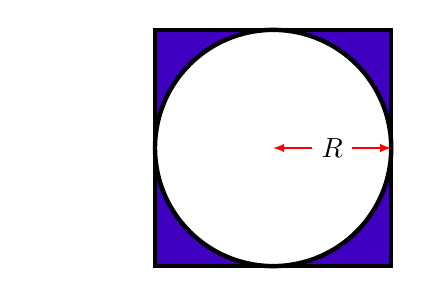
\begin{tikzpicture}[x=15mm,y=15mm,>=latex]
      \draw[black,ultra thick,fill=blue!75!red] (0,0) rectangle (2,2);
      \draw[black,ultra thick,fill=white] (1,1) circle (1);
      \draw[thin,red,<->] (1,1) -- (2,1) node[midway,black,fill=white] {$R$};
      \node at (-1,1) {\ };
    \end{tikzpicture}
  \end{minipage}
  \hfill
  \begin{minipage}{0.45\linewidth}
    \begin{align*}
      \text{A} & = \text{I have an answer}\\[0.5em]
      \text{B} & = \text{I know what to do}\\[0.5em]
      \text{C} & = \text{I am thinking}\\[0.5em]
      \text{D} & = \text{I do not know where to start}
    \end{align*}
  \end{minipage}
  \smallskip
  \pause

  \alert{Answer?}
  \pause

  The side of the square is $2R$, so the square has area $(2R)^2 =
  4R^2$.

  The area of the circle is $\pi R^2$.

  The shaded area is {\red$4R^2 - \pi R^2$}\ or {\red$(4-\pi)R^2$}.

  \begin{center}
    A$=$got it
    \quad 
    B$=$close
    \quad 
    C$=$not so close
  \end{center}

}

\frame{
  \frametitle{Review Question \#4}

  A bottle with {\blue\textsc{drink me}} written on it contains $50\%$ pure
  water and $50\%$ {\blue magicerium.} Alice wishes to add some of
  this to $7$ liters of pure water to obtain a {\red brew} which is
  $\red 20\%$ {\blue magicerium} and the rest pure water. How many
  liters should she take from the bottle labelled {\blue\textsc{drink me}}?
  \begin{center}
    A$ = 7$
    \quad 
    B$ = 14$
    \quad 
    C$ = 14/3$
    \quad 
    D$ = 7/3$
    \quad 
    E$ = 20$
    \pause
    \quad 
    \fbox{C}
  \end{center}
  \vspace*{2in}

}


\frame{
  \frametitle{Short Review Questions}

  \begin{itemize}
  \item[\red(1)]  What is the slope of the line $2y-3x=5$? 
    \begin{center}
      A$=3$
      \quad 
      B$ = -3$
      \quad 
      C$ = 2/3$
      \quad 
      D$=3/2$
      \quad 
      E$ = -3/2$
      \quad
      \pause
      \fbox{D}
    \end{center}
    \bigskip

    \item[\red(2)]  What is the $x$-coordinate of the point where the lines
      \begin{equation*}
        y+x=5
        \qquad\text{and}\qquad
        y=3x-2
      \end{equation*}
      intersect?

      \begin{center}
        A$=-1/3$
        \quad 
        B$=1/3$
        \quad 
        C$ = 3/4$
        \quad 
        D$ = 7/4$
        \quad
        \pause
        \fbox{D}
      \end{center}
      \bigskip
      
    \item[\red(3)] Solve {\Large$\frac{2^{\red x}}{3^{2{\red x}}}=5$}.
      
      \begin{center}
        A$= \log(5)/\log(2/3)$
        \quad 
        B$=\log(5)/(\log(2)-\log(3))$\\
        C$=\log(5)/(\log(2)+2\log(3))$
        \quad 
        D$=\log(5)/(\log(2)-2\log(3))$
        \quad
        \pause
        \fbox{D}
        \end{center}

  \end{itemize}

}



\frame{
  \frametitle{Lake Cachuma {\small(a linear approximation)}}
  % From {\red http://www.montecitowater.com/Sources_of_water.htm}
  \begin{itemize}
  \item Lake Cachuma was completed in 195{\red 0}.  \hfill{ \it
      \tiny{really completed 195{\red 3}}}

  \item It originally had a capacity of 205,000 acre feet ({\blue this
      is volume}). 

  \item In 2010 it has a capacity of approximately 190,000 acre-feet
    as a result of the accumulation of silt in the reservoir.

  \item ${\blue f(t)} = \text{{\blue{}capacity} in acre-feet of
      Cachuma lake $t$ years after 195{\red 0}}$. 
  \end{itemize}
  \gap

  \alert{(1)}\ Write down a linear approximation from this
  information for $\blue f(t)$. 
  \begin{center}
    A$ = 205,000-15,000t$
    \quad 
    B$ = 190,000+250t$
    \quad 
    C$ = 205,000-250t$\\[0.5em]
    %
    \ \quad
    D$ = 190,000-250t$
    \quad
    E$ = 190,000-125t$
    \quad
    \pause
    \fbox{C}
  \end{center}
  \vspace{.05in} 

  % Change in volume is $190000-205000=-15000.$ Change in time is
  % $2010-1950=60$ years. Average rate of change = $-15000/60=-250.$ So
  % Linear approximation is $f(t)=-250t+{\red b}.$ But
  % $f(0)=205000={\red b}.$ So \fbox{$f(t)=205000-250t$}
  % \vspace{.05in} 

  \alert{(2)}\ Which of the following years is the best
  estimate for when $10\%$\ of its original capacity will have been
  lost due to silt?
  \begin{center}
    A$= 2027$
    \quad 
    B$ = 2032$
    \quad 
    C$ = 2037$
    \quad 
    D$ = 2042$
    \quad 
    E$ = 2047$
    \pause
    \quad
    \fbox{B}
  \end{center}

}

\frame{

MISSING FIELD.PDF

A field has area 5000 square meters. It is surrounded by a wood fence that costs \$6 per meter length. It is divided in half by a brick wall that costs \$15 per meter length. Express the total costs of the wall and fence in terms of  $x=$ length of the wall in meters.

\gap
$A = 5000x\quad B = 15x+12W\quad C = 27x + 60000/x$\\
$ D = 15x + 30000/x\quad E = {\red hint}$\pause\\
Draw a {\red PLP} ={\red P}retty {\red L}ittle {\red P}icture\\
Name (and label on {\red PLP}) unknowns (length, width )\\
Get formula for {\blue cost} ({\purple of what exactly ?}) in terms of length and width\\
use given information to eliminate the dimension you don't want.




}

\frame{

MISSING FIELD2.PDF

A field has area 5000 square meters. It is surrounded by a wood fence that costs \$6 per meter length. It is divided in half by a brick wall that costs \$15 per meter length. Express the total costs of the wall and fence in terms of  $x=$ length of the wall in meters.

\gap
$A = 5000x\quad B = 15x+12W\quad C = 27x + 60000/x$\\
$ D = 15x + 30000/x$\quad\fbox{\blue C}

\gap $W=$ length of side of field perpendicular to brick wall.\\
$C=$ total cost =(cost brick)+(cost fence) \\
(cost brick) $=15x$\qquad (cost fence)=$6(2x+2W)=12x+12W$\\
$\therefore\quad C=15x+(12x+12)=27x+12W$\\
Area of field $=5000=xW$ so $W=5000/x.$\\
 Substitute for $W$ in above get $C=27x+12(5000/x)=27x+60000/x$


}

\frame{

An airline normally sells 3000  tickets per week on a certain route for \$200. When it has a sale, for every \$5 the price is lowered the number of tickets sold on the route increases by 60. Suppose the price is reduced by $5n$ dollars to \$(200-5n). How many tickets are sold ?\\
$A = 3000\quad B = 60\times (200-5n)\quad C =3000+(200-5n)\times 60$\\
$D = 3000+60n\quad E = 3000+12n$\pause\quad\fbox{\blue D}

\gap Reducing price \$$5n$ increases number of tickets by $60n$ to give total number of tickets = \fbox{$3000+60n$}

\gap If the ticket price is \$x how many tickets are sold?\\
$A = 3000-12x\quad B = 3000-60(200-x)\quad C = 5400-12x $\\
$ D = 3000+12x\quad E = 600+12x$\pause\quad\fbox{\blue C}

\gap $x=200-5n.$ Solve for $x$ get $5n=200-x$ so $n=40-(x/5).$\\
Substitute into $3000+60n$ for $n$ get $3000+60(40-(x/5))=$\fbox{$5400-12x$}

}








\frame{

{\blue HW18} {\it In the year 1900, in the country Acirema, there were {\blue 100} Lawyers and 
3 million people. Every {\red 10} years, the number of Lawyers doubles, and the population 
increases by 2 million. Let {\green t} be the number of years after 1900. Thus t=3 corresponds 
to 1903. Find the equation involving {\green t} whose solution tells you in which year 20 percent 
of the population are Lawyers. }

\gap $L({\green t}) =$ number of lawyers after ${\green t}$ years\\
$P({\green t}) = $ number of people after ${\green t}$ years\\

\halfgap Told initial population is 3 million and increases by 2 million in 10 years\\
 so increases 200,000 in 1 year so\qquad
$P({\green t})=3,000,000+200,000{\green t}$\halfgap

Told doubling time for lawyers is ${\red K}=\red 10$ years\\ 
{\blue initial number} is {\blue 100} so\qquad\qquad\qquad
$L({\green t})={\blue 100}\times2^{{\green t}/\red 10}$\\
Have 20\% Lawyers when
$$\frac{L({\green t})}{P({\green t})}=0.2=\frac{{\blue 100}\times2^{{\green t}/\red 10}}{(3,000,000+200,000{\green t})}$$


}


\frame{ \frametitle{Review Problems} {\red(1)}\ An oil slick in the
  shape of a rectangle is expanding. After $t$ hours the length is
  $30t$ meters and the width is $50t$ meters. How quickly is the area
  increasing in $\text{m}^2/\text{hour}$ after $2$ hours?
  \begin{center}
    A$=800$
    \quad 
    B$ = 1500$
    \quad 
    C$= 3200$
    \quad 
    D$ = 6000$
    \quad 
    E$ = \text{Other}$
    \pause
    \quad
    \fbox{D}
  \end{center}
  \bigskip

  {\red(2)}\ Suppose $f'(1)= 4$ and $g'(1)= 3$.  What is the rate of
  change of $f(x)+2g(x)$ when $x=1$? 
  \begin{center}
    A $=3$
    \quad 
    B $=4$
    \quad 
    C $=7$
    \quad 
    D $=10$
    \quad 
    E $=14$
    \quad
    \pause
    \fbox{D}
  \end{center}
  \bigskip

}


\frame{
  \frametitle{More Review Problems}

  {\blue(a)}\ What is the $x$-coordinate of the point on the graph
  $y=2x^2+5x-7$ where the slope is $11$? 
  \begin{center}
    A $ = 1$
    \quad 
    B $= 3/2$
    \quad 
    C $= 2$
    \quad 
    D $=5/3$
    \quad 
    E $=  0$
    \pause
    \quad
    \fbox{B}
  \end{center}
  \bigskip

  {\blue(b)}\ What is the value of $x$ at the point on the graph
  $y=4x^2 + 16 x$ where the tangent line is horizontal?
  \begin{center}
    A$=2$
    \quad 
    B$ = 0$
    \quad 
    C$ = -2$
    \quad 
    D$ =-4$
    \pause
    \quad
    \fbox{C}
  \end{center}
  \bigskip

  {\blue(c)}\ $\displaystyle\frac{d}{dx}\left(\frac{3}{x^4}\right)=$?
  \begin{center}
    A$\displaystyle=\frac{3}{4x^3}$
    \quad 
    B$\displaystyle = \frac{12}{x^5}$
    \quad 
    C$\displaystyle = -\frac{3}{4x^3}$
    \quad 
    D$\displaystyle = -\frac{12}{x^5}$
    \pause
    \quad
    \fbox{D}
  \end{center}
  \bigskip


}

